\documentclass[12pt, a4paper, oneside, openright, titlepage]{book}
\usepackage[utf8]{inputenc}
\raggedbottom
\usepackage{import}


%%%%%%%%%%%%%%%%% Book Formatting Comments:

%%%%%%%%%%%%%%%%%%%%%%%%%%%%%%%%%%%%% for Part

%%%%%%%%%%%%%%%%%%%%%% for chapter

%%%%%%%%%%%%%%%%%%%% for section








%%%%%% PACKAGES %%%%%%%
\usepackage{hyperref}
\hypersetup{
    colorlinks,
    citecolor=black,
    filecolor=black,
    linkcolor=black,
    urlcolor=black
}
\usepackage{amsmath} % Math display options
\usepackage{amssymb} % Math symbols
\usepackage{amsfonts} % Math fonts
\usepackage{amsthm}
\usepackage{mathtools} % General math tools
\usepackage{array} % Allows you to write arrays
\usepackage{empheq} % For boxing equations
\usepackage{mathabx}
\usepackage{mathrsfs}
\usepackage{nameref}

\usepackage{soul}
\usepackage[normalem]{ulem}

\usepackage{txfonts}
\usepackage{cancel}
\usepackage[toc, page]{appendix}
\usepackage{titletoc,tocloft}
\setlength{\cftchapindent}{1em}
\setlength{\cftsecindent}{2em}
\setlength{\cftsubsecindent}{3em}
\setlength{\cftsubsubsecindent}{4em}
\usepackage{titlesec}

\titleformat{\section}
  {\normalfont\fontsize{25}{15}\bfseries}{\thesection}{1em}{}
\titleformat{\section}
  {\normalfont\fontsize{20}{15}\bfseries}{\thesubsection}{1em}{}
\setcounter{secnumdepth}{1}  
  
  

\newcommand\numberthis{\refstepcounter{equation}\tag{\theequation}} % For equation labelling
\usepackage[framemethod=tikz]{mdframed}

\usepackage{tikz} % For drawing commutative diagrams
\usetikzlibrary{cd}
\usetikzlibrary{calc}
\tikzset{every picture/.style={line width=0.75pt}} %set default line width to 0.75p

\usepackage{datetime}
\usepackage[margin=1in]{geometry}
\setlength{\parskip}{1em}
\usepackage{graphicx}
\usepackage{float}
\usepackage{fancyhdr}
\setlength{\headheight}{15pt} 
\pagestyle{fancy}
\lhead[\leftmark]{}
\rhead[]{\leftmark}

\usepackage{enumitem}

\usepackage{url}
\allowdisplaybreaks

%%%%%% ENVIRONMENTS %%%
\definecolor{purp}{rgb}{0.29, 0, 0.51}
\definecolor{bloo}{rgb}{0, 0.13, 0.80}



%%\newtheoremstyle{note}% hnamei
%{3pt}% hSpace above
%{3pt}% hSpace belowi
%{}% hBody fonti
%{}% hIndent amounti
%{\itshape}% hTheorem head fonti
%{:}% hPunctuation after theorem headi
%{.5em}% hSpace after theorem headi
%{}% hTheorem head spec (can be left empty, meaning ‘normal’)i


%%%%%%%%%%%%% THEOREM STYLES

\newtheoremstyle{BigTheorem}
{20pt}
{20pt}
{\slshape}
{}
{\Large\color{purp}\bfseries}
{.}
{\newline}
{\thmname{#1}\thmnumber{ #2}\thmnote{ (#3)}}



\newtheoremstyle{TheoremClassic}
{15pt}
{15pt}
{\slshape}
{}
{\bfseries}
{.}
{.5em}
{}

\newtheoremstyle{Definitions}
{15pt}
{15pt}
{\slshape}
{}
{\bfseries}
{.}
{.5em}
{\thmname{#1}\thmnumber{ #2}\thmnote{ (#3)}}


\newtheoremstyle{Remarks}
{10pt}
{10pt}
{\upshape}
{}
{\bfseries}
{.}
{.5em}
{}

\newtheoremstyle{Examples}
{10pt}
{10pt}
{\upshape}
{}
{\bfseries}
{.}
{.5em}
{}


%%%%%%%%%%%%% THEOREM DEFINITIONS

\theoremstyle{BigTheorem}
\newtheorem{namthm}{Theorem}
\newtheorem{conj}[namthm]{Conjecture}

\theoremstyle{TheoremClassic}
\newtheorem{thm}{Theorem}[section]
\newtheorem*{thm*}{Theorem}
\newtheorem{lem}[thm]{Lemma}
\newtheorem{cor}[thm]{Corollary}
\newtheorem{prop}[thm]{Proposition}
\newtheorem{claim}[thm]{Claim}


\theoremstyle{Definitions}
\newtheorem{defn}{Definition}[section]
\newtheorem{axi}[defn]{Axiom}
\newtheorem{cust}[defn]{}
\newtheorem{cons}[defn]{Construction}
\newtheorem{props}[defn]{Properties}
\newtheorem{proc}[defn]{Process}
\newtheorem*{law}{Law}


\theoremstyle{Examples}
\newtheorem{eg}{Example}[section]
\newtheorem{noneg}[eg]{Non-Example}
\newtheorem{xca}[eg]{Exercise}


\theoremstyle{Remarks}
\newtheorem{rmk}{Remark}[section]
\newtheorem{qst}[rmk]{Question}
\newtheorem*{ans}{Answer}
\newtheorem{obs}[rmk]{Observation}
\newtheorem{rec}[rmk]{Recall}
\newtheorem{summ}[rmk]{Summary}
\newtheorem{nota}[rmk]{Notation}
\newtheorem{note}[rmk]{Note}



\renewcommand{\qedsymbol}{$\blacksquare$}


\numberwithin{equation}{section}

\newenvironment{qest}{
    \begin{center}
        \em
    }
    {
    \end{center}
    }

%%%%%% MACROS %%%%%%%%%
%% New Commands
\newcommand{\ip}[1]{\langle#1\rangle} %%% Inner product
\newcommand{\abs}[1]{\lvert#1\rvert} %%% Modulus
\newcommand\diag{\operatorname{diag}} %%% diag matrix
\newcommand\tr{\mbox{tr}\.} %%% trace
\newcommand\C{\mathbb C} %%% Complex numbers
\newcommand\R{\mathbb R} %%% Real numbers
\newcommand\Z{\mathbb Z} %%% Integers
\newcommand\Q{\mathbb Q} %%% Rationals
\newcommand\N{\mathbb N} %%% Naturals
\newcommand\F{\mathbb F} %%% An arbitrary field
\newcommand\ste{\operatorname{St}} %%% Steinberg Representation
\newcommand\GL{\mathbf{GL}} %%% General Linear group
\newcommand\SL{\mathbf{SL}} %%% Special linear group
\newcommand\gl{\mathfrak{gl}} %%% General linear algebra
\newcommand\G{\mathbf{G}} %%% connected reductive group
\newcommand\g{\mathfrak{g}} %%% Lie algebra of G
\newcommand\Hbf{\mathbf{H}} %%% Theta fixed points of G
\newcommand\X{\mathbf{X}} %%% Symmetric space X
\newcommand{\catname}[1]{\normalfont\textbf{#1}}
\newcommand{\Set}{\catname{Set}} %%% Category set
\newcommand{\Grp}{\catname{Grp}} %%% Category group
\newcommand{\Rmod}{\catname{R-Mod}} %%% Category r-modules
\newcommand{\Mon}{\catname{Mon}} %%% Category monoid
\newcommand{\Ring}{\catname{Ring}} %%% Category ring
\newcommand{\Topp}{\catname{Top}} %%% Category Topological spaces
\newcommand{\Vect}{\catname{Vect}_{k}} %%% category vector spaces'
\newcommand\Hom{\mathbf{Hom}} %%% Arrows

\newcommand{\map}[2]{\begin{array}{c} #1 \\ #2 \end{array}}

\newcommand{\Emph}[1]{\textbf{\ul{\emph{#1}}}}

\newcommand{\mapsfrom}{\mathrel{\reflectbox{\ensuremath{\mapsto}}}}


%% Math operators
\DeclareMathOperator{\ran}{Im} %%% image
\DeclareMathOperator{\aut}{Aut} %%% Automorphisms
\DeclareMathOperator{\spn}{span} %%% span
\DeclareMathOperator{\ann}{Ann} %%% annihilator
\DeclareMathOperator{\rank}{rank} %%% Rank
\DeclareMathOperator{\ch}{char} %%% characteristic
\DeclareMathOperator{\ev}{\bf{ev}} %%% evaluation
\DeclareMathOperator{\sgn}{sign} %%% sign
\DeclareMathOperator{\id}{Id} %%% identity
\DeclareMathOperator{\supp}{Supp} %%% support
\DeclareMathOperator{\inn}{Inn} %%% Inner aut
\DeclareMathOperator{\en}{End} %%% Endomorphisms
\DeclareMathOperator{\sym}{Sym} %%% Group of symmetries


%% Diagram Environments
\iffalse
\begin{center}
    \begin{tikzpicture}[baseline= (a).base]
        \node[scale=1] (a) at (0,0){
          \begin{tikzcd}
           
          \end{tikzcd}
        };
    \end{tikzpicture}
\end{center}
\fi




\newdateformat{monthdayyeardate}{%
    \monthname[\THEMONTH]~\THEDAY, \THEYEAR}
%%%%%%%%%%%%%%%%%%%%%%%

%%% Specific Macros %%%


%%%%%% BEGIN %%%%%%%%%%


\begin{document}

%%%%%% TITLE PAGE %%%%%

\begin{titlepage}
    \centering
    \scshape
    \vspace*{\baselineskip}
    \rule{\textwidth}{1.6pt}\vspace*{-\baselineskip}\vspace*{2pt}
    \rule{\textwidth}{0.4pt}
    
    \vspace{0.75\baselineskip}
    
    {\LARGE Mathematical Physics: A Complete Guide}
    
    \vspace{0.75\baselineskip}
    
    \rule{\textwidth}{0.4pt}\vspace*{-\baselineskip}\vspace{3.2pt}
    \rule{\textwidth}{1.6pt}
    
    \vspace{2\baselineskip}
    Phys 435 \\
    \vspace*{3\baselineskip}
    \monthdayyeardate\today \\
    \vspace*{5.0\baselineskip}
    
    {\scshape\Large Elijah Thompson, \\ Physics and Math Honors\\}
    
    \vspace{1.0\baselineskip}
    \textit{Solo Pursuit of Learning}
    \vfill
    \enlargethispage{1in}
    \begin{figure}[b!]
    \makebox[\textwidth]{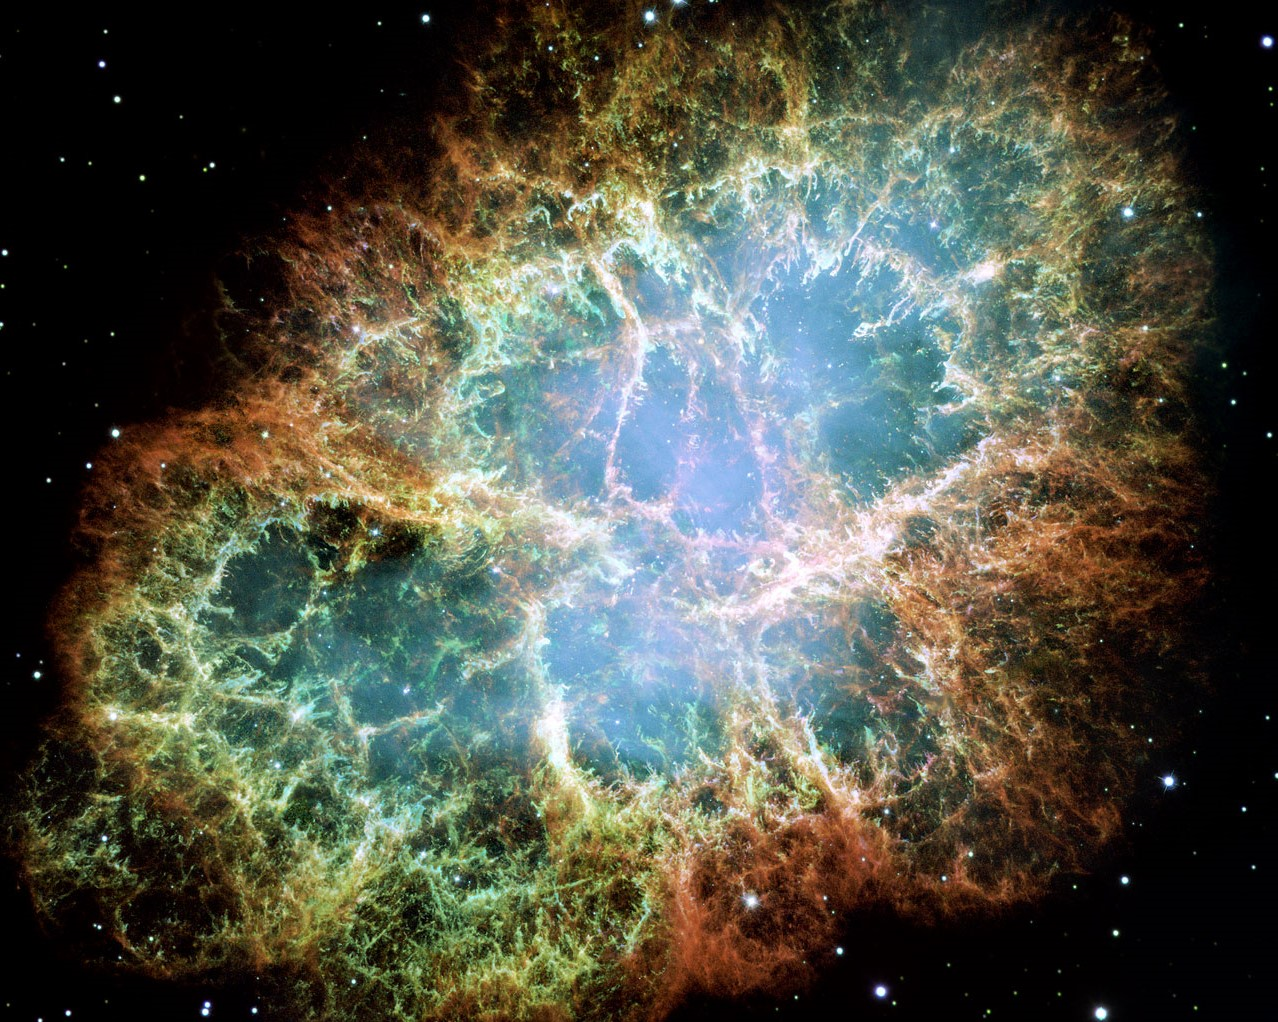
\includegraphics[width=\paperwidth, height =10cm]{../Crab.jpg}}
    \end{figure}
\end{titlepage}

%%%%%%%%%%%%%%%%%%%%%%%
\tableofcontents



%%%%%%%%%%%%%%%%%%%%%%%%%%%%%%%%%%%%% Part 1
\part{Complex Analysis}


%%%%%%%%%%%%%%%%%%%%%% Chapter 1.1
\chapter{Properties of Complex Functions}

%%%%%%%%%%%%%%%%%%%% Section 1.1.1
\section{Elementary Definitions}


%%%%%%%%%%%%%%%%%%%% Section 1.1.2
\section{Multivalued Functions and Branch Cuts}


%%%%%%%%%%%%%%%%%%%% Section 1.1.3
\section{Analytic Functions and the Cauchy-Riemann Equations}


%%%%%%%%%%%%%%%%%%%% Section 1.1.4
\section{Singularities and Zeros}


%%%%%%%%%%%%%%%%%%%% Section 1.1.5
\section{Conformal Mappings}


%%%%%%%%%%%%%%%%%%%%%% Chapter 1.2
\chapter{Power Series and Laurent Series}


%%%%%%%%%%%%%%%%%%%% Section 1.2.1
\section{Power Series Fundamentals}


%%%%%%%%%%%%%%%%%%%% Section 1.2.2
\section{Laurent Series}


%%%%%%%%%%%%%%%%%%%% Section 1.2.3
\section{Series Operations}



%%%%%%%%%%%%%%%%%%%%%% Chapter 1.3
\chapter{Complex Integration}

%%%%%%%%%%%%%%%%%%%% Section 1.3.1
\section{Complex Integral}


%%%%%%%%%%%%%%%%%%%% Section 1.3.2
\section{Cauchy's Theorems}


%%%%%%%%%%%%%%%%%%%% Section 1.3.3
\section{Residue Theorem}


%%%%%%%%%%%%%%%%%%%% Section 1.3.4
\section{Contour Integrals}


%%%%%%%%%%%%%%%%%%%%%% Chapter 1.4
\chapter{Applications of Complex Functions}


%%%%%%%%%%%%%%%%%%%% Section 1.4.1
\section{Complex Potentials}


%%%%%%%%%%%%%%%%%%%% Section 1.4.2
\section{Finding Zeros}


%%%%%%%%%%%%%%%%%%%% Section 1.4.3
\section{Inverse Laplace}

%%%%%%%%%%%%%%%%%%%% Section 1.4.4
\section{Stokes' Equations and Airy Integrals}


%%%%%%%%%%%%%%%%%%%% Section 1.4.5
\section{WKB Methods, and Integral Approximations}




%%%%%%%%%%%%%%%%%%%%%%%%%%%%%%%%%%%%% Part 2
\part{PDEs}


%%%%%%%%%%%%%%%%%%%%%% Chapter 2.1
\chapter{General and Particular Solutions}

%%%%%%%%%%%%%%%%%%%% Section 2.1.1
\section{Important Examples and Motivation}



%%%%%%%%%%%%%%%%%%%% Section 2.1.2
\section{General Forms of Solutions}



%%%%%%%%%%%%%%%%%%%% Section 2.1.3
\section{Wave and Diffusion Equations}



%%%%%%%%%%%%%%%%%%%% Section 2.1.4
\section{Existence and Uniqueness}




%%%%%%%%%%%%%%%%%%%%%% Chapter 2.2
\chapter{Fourier Series}


%%%%%%%%%%%%%%%%%%%% Section 2.2.1
\section{Initial Definitions and Dirichlet Conditions}


\begin{defn}
    Sufficients conditions for which a function $f(x)$ to have its Fourier series to converge to it are known as the \Emph{Dirichlet conditions}: \begin{enumerate}
        \item[(i)] $f(x)$ must be periodic; i.e. there exists $p \in \R$ such that $f(x+p) = f(x)$ for all $x \in \R$.
        \item[(ii)] $f(x)$ must be continuous, except possibly at a finite number of jump (i.e. finite) discontinuities in any bounded interval.
        \item[(iii)] $f(x)$ must be of \Emph{bounded variation} on any bounded interval, which is to say its total variation is finite; if $f$ is differentiable and its derivative is Riemann-integrable on the interval, then the total variation is the absolute integral of the derivative over the interval: $$V_a^b(f) = \int_a^b|f'(x)|dx$$
            An alternative formulation is to require that any bounded interval contains only a finite number of extrema of $f$.
        \item[(iv)] $f(x)$ is absolutely integrable over a period, so $$\int_0^p|f(x)|dx < \infty$$
    \end{enumerate}
    If these criterions hold, the Fourier series converges to $f(x)$ at all points where the function is continuous.
\end{defn}

Recall that a function $f(x)$ can be split into an even and odd part: \begin{equation*}
    f(x) = \frac{1}{2}[f(x) + f(-x)] + \frac{1}{2}[f(x) - f(-x)] = f_{even}(x) + f_{odd}(x)
\end{equation*}
Then, we can write the even component as a cosine series and the odd component as a sine series.

\begin{prop}
    For any $L \in \R$, the set of functions \begin{equation*}
        \left\{1,\cos\frac{2\pi x}{L},\sin\frac{2\pi x}{L},\cos\frac{2\pi 2x}{L},\sin\frac{2\pi 2x}{L},...,\cos\frac{2\pi nx}{L},\sin\frac{2\pi nx}{L},...\right\}
    \end{equation*}
    form an orthogonal set with respect to the inner product \begin{equation*}
        \langle f,g\rangle = \int_{x_0}^{x_0+L}f(x)g(x)dx
    \end{equation*}
    for $x_0 \in \R$ fixed. In particular, we have \begin{align*}
        \int_{x_0}^{x_0+L}\sin\frac{2\pi nx}{L}\cos\frac{2\pi mx}{L}dx &= 0,\;\;\forall n,m \in \N\cup \{0\} \\
        \int_{x_0}^{x_0+L}\cos\frac{2\pi nx}{L}\cos\frac{2\pi mx}{L}dx &= \left\{\begin{array}{lc} L & \text{if } n = m = 0, \\ \frac{L}{2} & \text{if } n = m > 0, \\ 0 & \text{if } n \neq m \end{array}\right. \\
        \int_{x_0}^{x_0+L}\sin\frac{2\pi nx}{L}\sin\frac{2\pi mx}{L}dx &= \left\{\begin{array}{lc} 0 & \text{if } n = m = 0, \\ \frac{L}{2} & \text{if } n = m > 0, \\ 0 & \text{if } n \neq m \end{array}\right. \\
    \end{align*}
\end{prop}


\begin{defn}
    The classical Fourier series expansion of a function $f(x)$ is \begin{equation}
        f(x) \sim \frac{a_0}{2} + \sum_{n=1}^{\infty}\left[a_n\cos\frac{2\pi xn}{L}+b_n\sin\frac{2\pi nx}{L}\right]
    \end{equation}
    where $a_0,a_n,b_n$, for $n \geq 1$, are called the \Emph{Fourier coefficients}
\end{defn}

For a periodic function $f(x)$ of period $L$, we use the orthogonality conditions to find the Fourier coefficients as follows: \begin{align}
    a_0 &= \frac{2}{L}\int_{x_0}^{x_0+L}f(x)\cdot 1dx \\
    a_n &= \frac{2}{L}\int_{x_0}^{x_0+L}f(x)\cdot \cos\frac{2\pi nx}{L}dx \\
    b_n &= \frac{2}{L}\int_{x_0}^{x_0+L}f(x)\cdot \sin\frac{2\pi nx}{L}dx
\end{align}
where $x_0$ is arbitrary, but fixed, and $n \geq 1$.


\subsection{Symmetry Conditions}

From these coefficient equations we observe that if $f(x)$ is even with respect to the origin then all sine terms, $b_n$, are zero. Conversely, if $f(x)$ is odd with respect to the origin then all cosine terms, $a_n$, are zero. We now consider a more subtle symmetry about $L/4$, where $L$ is a period of $f$, so $f(x+L) = f(x)$ for all $x \in \R$.

\begin{defn}
    We say that $f(x)$ has even symmetry about $L/4$ if $f(L/4-x) = f(x-L/4)$ for all $x \in \R$. We say that $f(x)$ has odd symmetry about $L/4$ if $f(L/4-x) = -f(x-L/4)$.
\end{defn}

We consider the sine terms of $g(x) = f(x-L/4)$, and substitute $s = x-L/4$: \begin{align*}
    b_n &= \frac{2}{L}\int_{x_0}^{x_0+L}f(x-L/4)\sin\frac{2\pi nx}{L}dx \\
    &= \frac{2}{L}\int_{x_0-L/4}^{x_0-L/4+L}f(s)\sin\left[\frac{2\pi ns}{L} + \frac{\pi n}{2}\right]ds \\
    &= \frac{2}{L}\int_{x_0}^{x_0+L}f(s)\sin\left[\frac{2\pi ns}{L} + \frac{\pi n}{2}\right]ds
\end{align*}
where the limits of integration can be changed since $f$ is periodic. We observe that \begin{equation*}
    \sin\left[\frac{2\pi ns}{L} + \frac{\pi n}{2}\right] = \sin\frac{2\pi ns}{L}\cos\frac{\pi n}{2}+\cos\frac{2\pi ns}{L}\sin\frac{\pi n}{2}
\end{equation*}
so the trigonometric portion of the integrand is odd if $n$ is even and even if $n$ is odd. Then if $f(s)$ is even and $n$ is even the integral is zero, and similarly if $f(s)$ is odd and $n$ is odd the integral is zero. For the cosine coefficients we have \begin{equation*}
    \cos\left[\frac{2\pi ns}{L} + \frac{\pi n}{2}\right] = \cos\frac{2\pi ns}{L}\cos\frac{\pi n}{2}-\sin\frac{2\pi ns}{L}\sin\frac{\pi n}{2}
\end{equation*}
which is even if $n$ is even and odd if $n$ is odd. Then if $f(s)$ is even and $n$ is odd, the terms $a_n$ are zero, and if $f(s)$ is odd and $n$ is even, the terms $a_n$ are zero. In summary: \begin{itemize}
    \item If $f(x)$ is even about $L/4$, then $a_{2n-1} = 0$ and $b_{2n} = 0$ for all $n \geq 1$,
    \item If $f(x)$ is odd about $L/4$, then $a_{2n} = 0$ and $b_{2n+1} = 0$ for all $n \geq 0$.
\end{itemize}


%%%%%%%%%%%%%%%%%%%% Section 2.2.3
\section{Discontinuous and Non-Periodic Functions}

\subsection{Discontinuities}

\begin{defn}
    The error term for the Fourier series representation of $f$ when expressed as a partial sum with highest term $N$ is \begin{equation*}
        E_N(x) = \left|f(x) - \left[\frac{a_0}{2}+\sum_{n=1}^N\left(a_n\cos\frac{2\pi nx}{L}+b_n\sin\frac{2\pi nx}{L}\right)\right]\right|
    \end{equation*}
\end{defn}

If $f(x)$ is discontinuous at a point $a$ in the domain of interest, then the Fourier series for $f(x)$ does not produce a discontinuity at $a$ but rather converges to the value \begin{equation*}
    \frac{1}{2}[f(a+)+f(a-)]
\end{equation*}
where $f(a+) = \lim\limits_{x\rightarrow a^+}f(x)$ is the one-sided limit from above, and $f(a-) = \lim\limits_{x\rightarrow a^-}f(x)$ is the one-sided limit from below. Then, there exists sequences $u_n$ and $v_n$ such that $u_n,v_n\rightarrow a$, with $u_n < a$ for all $n$ and $v_n > a$ for all $n$ and \begin{equation*}
    E_N(u_N) \approx 0.9|f(a-)-f(a+)|\;\;\;E_N(v_N) \approx 0.9|f(a-)-f(a+)|
\end{equation*}
so the maximum value of the error $E_N(x)$ near $a$ does not approach zero as $N\rightarrow \infty$, but rather occurs closer and closer to $a$, and is essentially independent of $N$. This is known as the \Emph{Gibbs' phenomenon}.


\subsection{Non-Periodic Functions}

We often wish to analysize non-periodic functions using Fourier analysis, and this can be done by using appropriate periodic extensions:

\begin{thm}
    Suppose $h$ is differentiable on $[0,L]$; that is, $h'(x)$ exists for $0 < x< L$, and the one-sided derivatives \begin{equation*}
        h'_+ = \lim\limits_{x\rightarrow 0^+}\frac{h(x)-h(0)}{x}\;\;\text{ and }\;\;h'_-(L) = \lim\limits_{x\rightarrow L^-}\frac{h(x) - h(L)}{x-L}
    \end{equation*}
    both exist. \begin{itemize}
        \item Let $O$ denote the odd periodic extension of $h$ to $(-\infty,\infty)$ defined by \begin{equation*}
                O(x) = \left\{\begin{array}{lc} h(x), & 0 \leq x \leq L \\ -h(-x), & -L < x < 0,\end{array}\right.\text{ and } O(x+2L) = O(x),\;\;\forall x \in \R
        \end{equation*}
            Then $O$ is differentiable on $(-\infty,\infty)$ if and only if \begin{equation*}
                h(0) = h(L) = 0
            \end{equation*}
        \item Let $E$ denote the even periodic extension of $h$ to $(-\infty, \infty)$, defined by \begin{equation*}
                E(x) = \left\{\begin{array}{lc} h(x), & 0 \leq x \leq L \\ h(-x), & -L < x < 0,\end{array}\right.\text{ and } E(x+2L) = E(x),\;\;\forall x \in \R
        \end{equation*}
            Then $E$ is differentiable on $(-\infty,\infty)$ if and only if \begin{equation*}
                h_+'(0) = h_-'(L) = 0
            \end{equation*}
    \end{itemize}
\end{thm}





%%%%%%%%%%%%%%%%%%%% Section 2.2.4
\section{Integration and Differentiation}

\begin{thm}
    If $f(x)$ satisfies the Dirichlet conditions, then integrating the Fourier series of $f(x)$ term by term produces a Fourier series which converges to the integral of $f(x)$, modulo an arbitrary constant.
\end{thm}

\begin{thm}
    If $f(x)$ satisfies the Dirichlet conditions, is differentiable, and $f'(x)$ satisfies the Dirichlet conditions, then the Fourier series obtained by differentiating $f$'s Fourier series term by term converges to $f'(x)$.
\end{thm}

For general functional series we have the following important result: 

\begin{thm}
    A convergent infinite series \begin{equation*}
        W(z) = \sum_{n=1}^{\infty}w_n(z)
    \end{equation*}
    can be differentiated term by term on a closed interval $[z_1,z_2]$ to obtain \begin{equation*}
        W'(z) = \sum_{n=1}^{\infty}w'_n(z)
    \end{equation*}
    provided that $w'_n$ is continuous on $[z_1,z_2]$ and there exists a sequence $M_n$ of constants such that $\sum_{n=1}^{\infty}M_n$ converges and \begin{equation*}
        |w'_n(z)| \leq M_n,\;\;z_1 \leq z \leq z_2,\;\;n=1,2,3,...
    \end{equation*}
\end{thm}


%%%%%%%%%%%%%%%%%%%% Section 2.2.5
\section{Complex Fourier Series}

Recall that by DeMoivre's Formula we have the following for the complex exponential: \begin{equation*}
    \exp\left\{ix\right\} = \cos x + i\sin x
\end{equation*}
\begin{defn}
    For a function $f(x)$ of period $L$, its complex Fourier series expansion is given by \begin{equation*}
        f(x) \sim \sum_{n=-\infty}^{\infty}c_n\exp\left\{\frac{2\pi inx}{L}\right\}
    \end{equation*}
\end{defn}

We remark that the set of functions $$\left\{1,\exp\left\{\frac{2\pi x}{L}\right\},\exp\left\{\frac{2\pi 2x}{L}\right\},...\exp\left\{\frac{2\pi nx}{L}\right\},...\right\}$$
forms an orthogonal set under the complex inner product \begin{equation*}
    \langle f, g\rangle = \int_{x_0}^{x_0+L}f(x)\overline{g(x)}dx
\end{equation*}
for $x_0$ fixed with the relation \begin{equation*}
    \int_{x_0}^{x_0+L}\exp\left\{\frac{2\pi inx}{L}\right\}\exp\left\{-\frac{2\pi imx}{L}\right\}dx = \left\{\begin{array}{lc} L & \text{if } m = n \\ 0 & \text{if } m \neq n\end{array}\right.
\end{equation*} 
Then the Fourier coefficients are given by \begin{equation}
    c_n = \frac{1}{L}\int_{x_0}^{x_0+L}f(x)\exp\left\{-\frac{2\pi inx}{L}\right\}dx
\end{equation}

We expand the complex exponential in the Fourier series as follows: \begin{align*}
    \sum_{n=-\infty}^{\infty}c_n\exp\left\{\frac{2\pi nx}{L}\right\} &= \sum_{n=1}^{\infty}c_{-n}\exp\left\{\frac{-2\pi nx}{L}\right\} + c_0 + \sum_{n=1}^{\infty}c_n\exp\left\{\frac{2\pi nx}{L}\right\} \\
    &= c_0 + \sum_{n=1}^{\infty}\left[c_{-n}\left(\cos\frac{2\pi nx}{L} - i\sin\frac{2\pi nx}{L}\right) + c_n\left(\cos\frac{2\pi nx}{L} - i\sin\frac{2\pi nx}{L}\right)\right] \\
    &= c_0 + \sum_{n=1}^{\infty}\left[(c_{-n}+c_n)\cos\frac{2\pi nx}{L}+(ic_n - ic_{-n})\sin\frac{2\pi nx}{L}\right]
\end{align*}
From this expansion we find that \begin{align*}
    c_0 &= \frac{a_0}{2} \\
    c_{-n}+c_n &= a_n \\
    ic_n - ic_{-n} &= b_n
\end{align*}
for $n \geq 1$. Then we have that \begin{equation*}
    c_n = \frac{1}{2}(a_n - ib_n) \;\;\text{ and }\;\;c_{-n} = \frac{1}{2}(a_n + ib_n)
\end{equation*}
It follows that if $f(x)$ is real, so $a_n$ and $b_n$ are real, $c_{-n} = \overline{c_n}$.


\subsection{Parseval's Theorem}

\begin{namthm}[Parseval's Theorem]
    Suppose that $A(x)$ and $B(x)$ are two complex valued functions on $\R$ of period $2L$ that are square integrable with respect to the Lebesgue measure over intervals of period length with complex Fourier series\begin{equation*}
        A(x) = \sum_{n=-\infty}^{\infty}a_n\exp\left\{\frac{i\pi nx}{L}\right\},\;\text{ and }\;B(x) = \sum_{n=-\infty}^{\infty}b_n\exp\left\{\frac{i\pi nx}{L}\right\}
    \end{equation*}
    Then \begin{equation}
        \sum_{n=-\infty}^{\infty}a_n\overline{b_n} = \frac{1}{2L}\int_{-L}^LA(x)\overline{B(x)}dx
    \end{equation}
\end{namthm}
\begin{proof}
    Suppose $A(x)$ and $B(x)$ are as above, with corresponding Fourier series, and observe that \begin{align*}
        \frac{1}{2L}\int_{-L}^LA(x)\overline{B(x)}dx &= \sum_{n=-\infty}^{\infty}a_n\frac{1}{2L}\int_{-L}^L\overline{B(x)}\exp\left\{\frac{2\pi inx}{2L}\right\}dx \\
        &= \sum_{n=-\infty}^{\infty}a_n\overline{\left[\frac{1}{2L}\int_{-L}^LB(x)\exp\left\{\frac{-2\pi inx}{2L}\right\}dx\right]} \\
        &= \sum_{n=-\infty}^{\infty}a_n\overline{b_n}
    \end{align*}
    as desired.
\end{proof}

As a corollary, we have that for any function $f(x)$ of period $L$, \begin{equation*}
    \frac{1}{L}\int_{x_0}^{x_0+L}|f(x)|^2dx = \sum_{n=-\infty}^{\infty}|c_n|^2 = \frac{|a_0|^2}{4} + \frac{1}{2}\sum_{n=1}^{\infty}(a_n^2+b_n^2)
\end{equation*}

This says that the sum of the moduli squared of the complex Fourier coefficients is equal to the average value of $|f(x)|^2$ over one period. 



%%%%%%%%%%%%%%%%%%%%%% Chapter 2.3
\chapter{Integral Transforms}


%%%%%%%%%%%%%%%%%%%% Section 2.3.1
\section{Fourier Transform}


%%%%%%%%%%%%%%%%%%%% Section 2.3.2
\section{Laplace Transform}




%%%%%%%%%%%%%%%%%%%%%% Chapter 2.4
\chapter{Separation of Variables and Other Methods}


%%%%%%%%%%%%%%%%%%%% Section 2.4.1
\section{Separation of Variables}



%%%%%%%%%%%%%%%%%%%% Section 2.4.2
\section{Applying Integral Transforms}



%%%%%%%%%%%%%%%%%%%% Section 2.4.3
\section{Inhomogeneous Problems}






%%%%%%%%%%%%%%%%%%%%%% - Appendices
\begin{appendices}


\end{appendices}


\end{document}


%%%%%% END %%%%%%%%%%%%%
